
\section{Example: Modeling Storglaci{\"a}ren, a mountain glacier}\label{sec:storglaciaren} \index{Storglaci{\"a}ren}
\optsection{Storglaci{\"a}ren}

Storglaci{\"a}ren is a small valley glacier in northern Sweden (Figure~\ref{fig:storglaciaren}). The glacier is approximately 3.2\,km long and 1\,km wide, therefore much smaller than a single grid cell in a typical Greenland model. By the way ``Storglaci{\"a}ren'' means ``big glacier'' in Swedish. Most of the glacier is temperate, except for a thin cold near-surface layer in the ablation zone. Such a thermal structure is often-called a Scandinavian-type structure. Thanks to the nearby Tarfala research station it is one of the best investigated glaciers worldwide, and the wealth of data available makes it perfectly suitable for all kinds of modeling studies. In this tutorial we demonstrate how PISM can be used for valley glaciers in a flow-line application. Additionally we show that PISM's conservation of energy scheme is able to simulate the glacier's thermal structure.

\begin{figure}[ht]
  \centering
  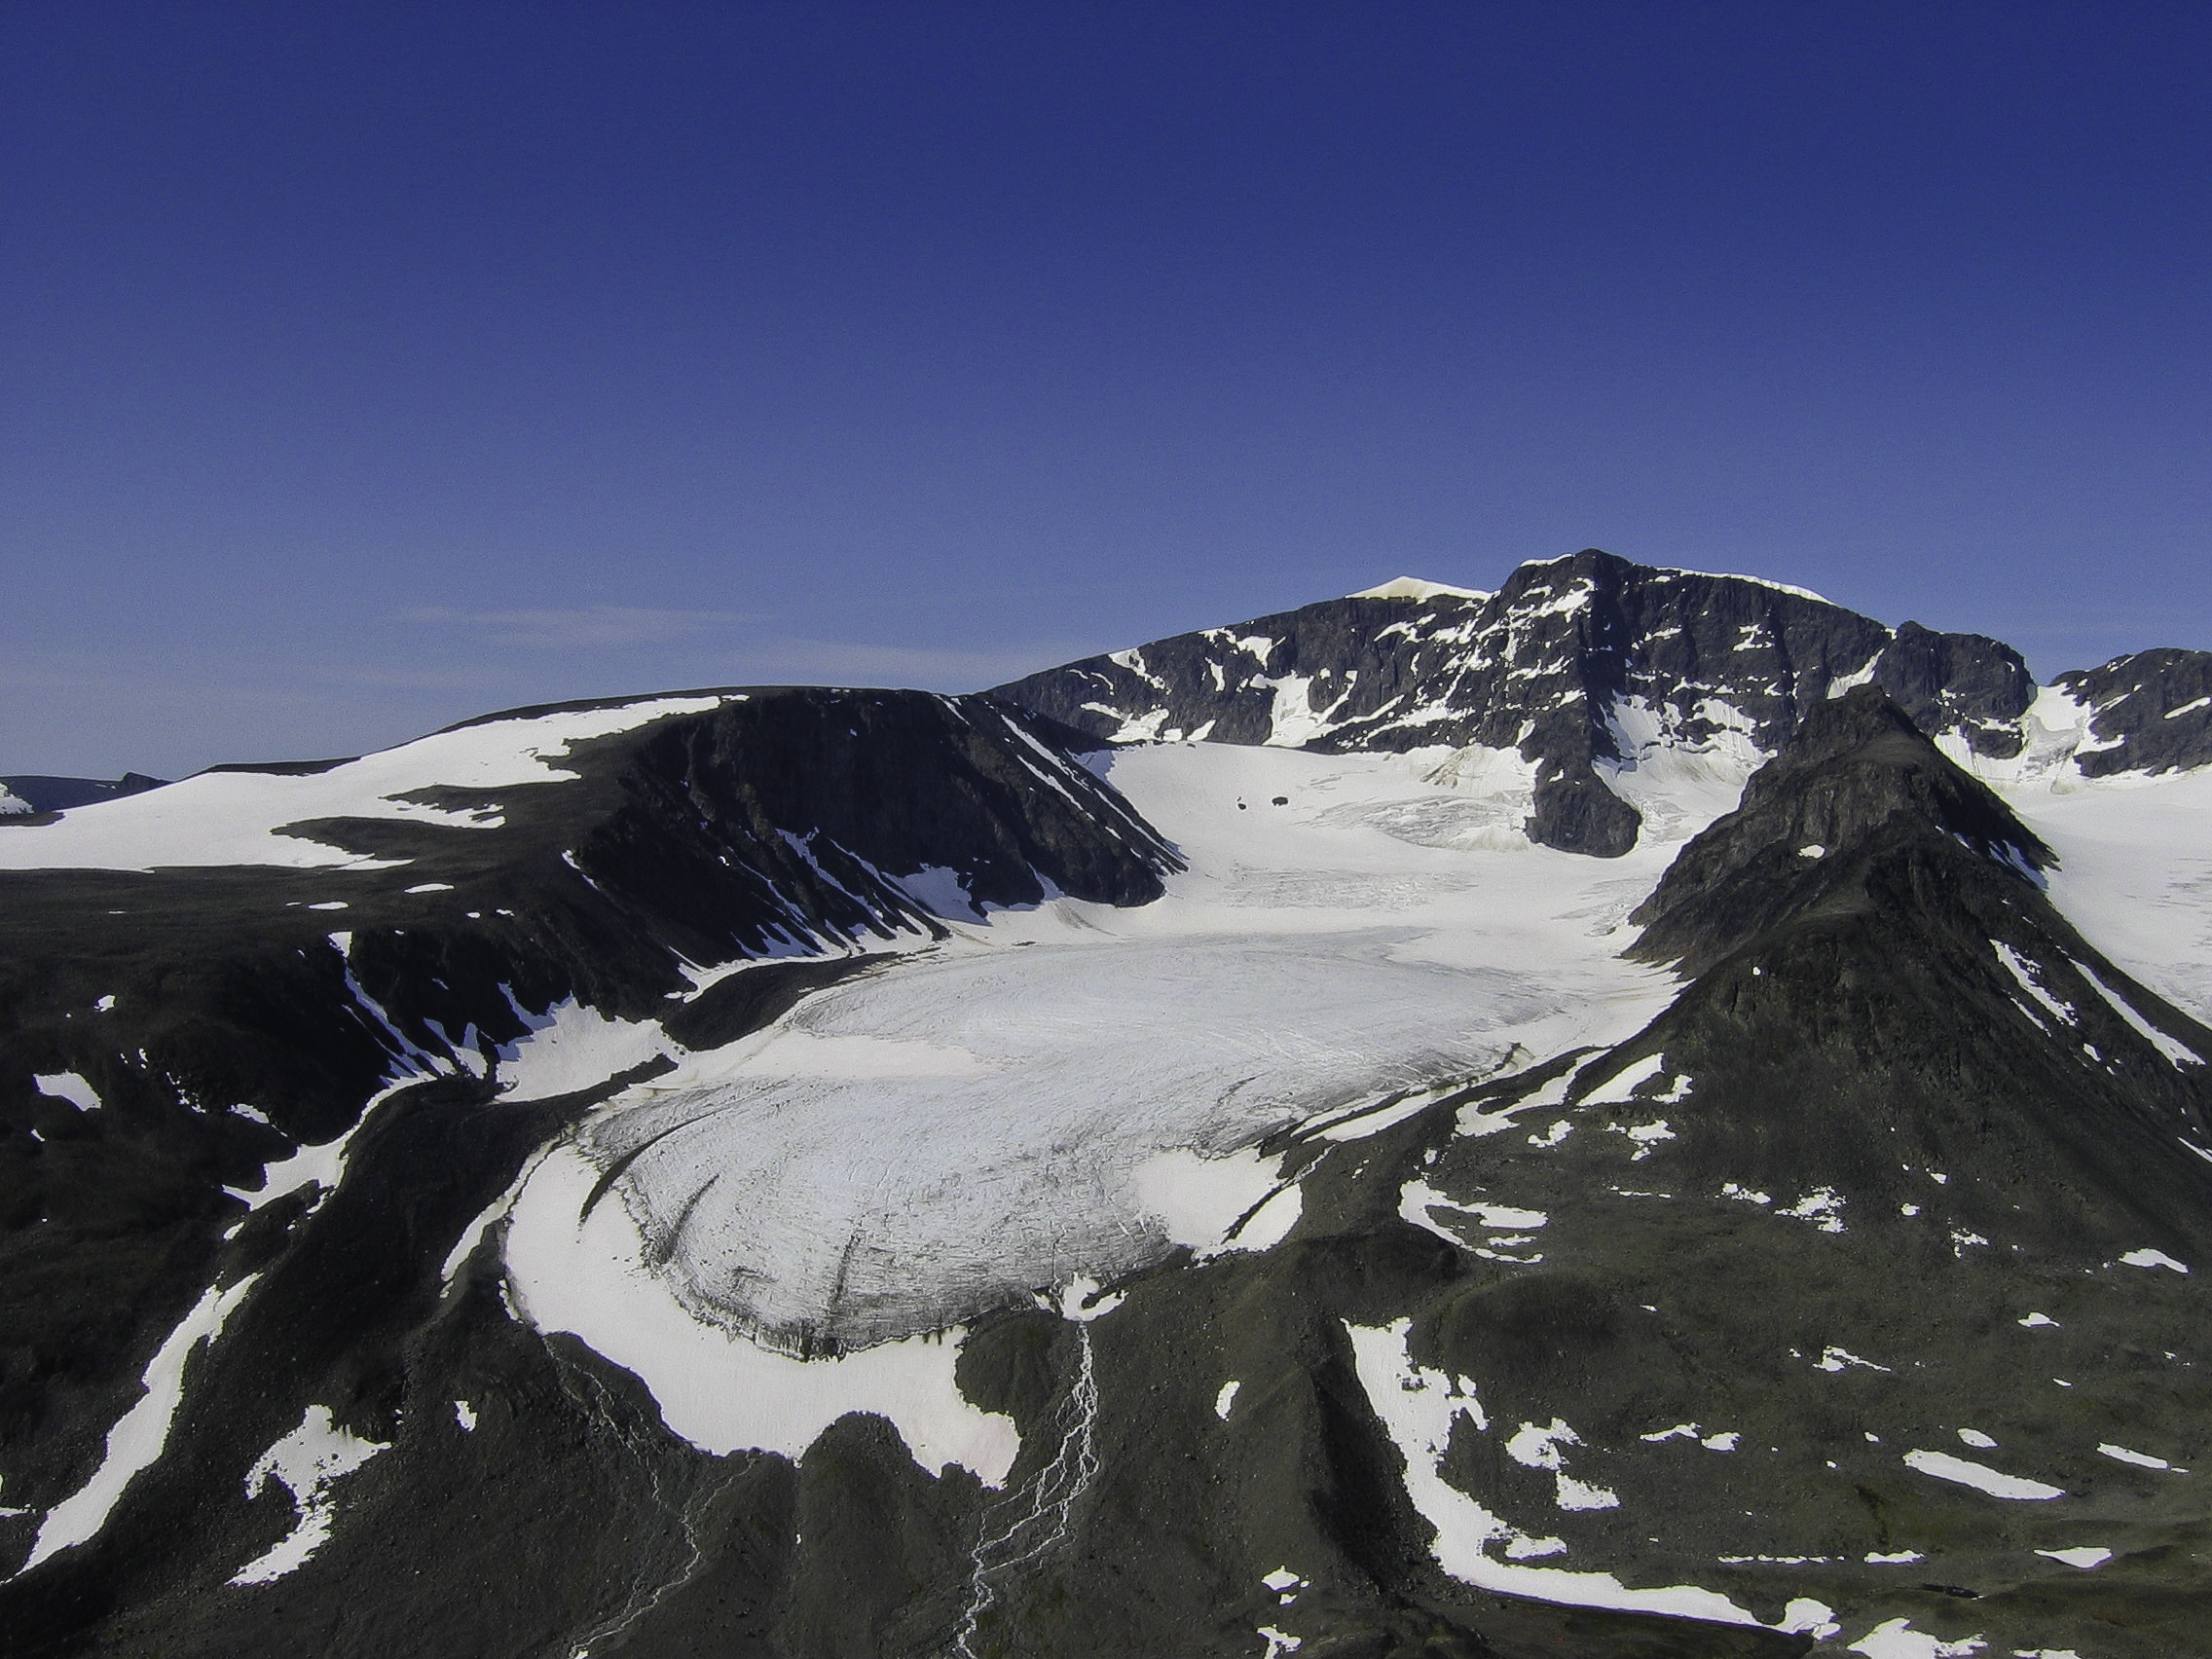
\includegraphics[width=3.in,keepaspectratio=true]{storglaciaren}\qquad
  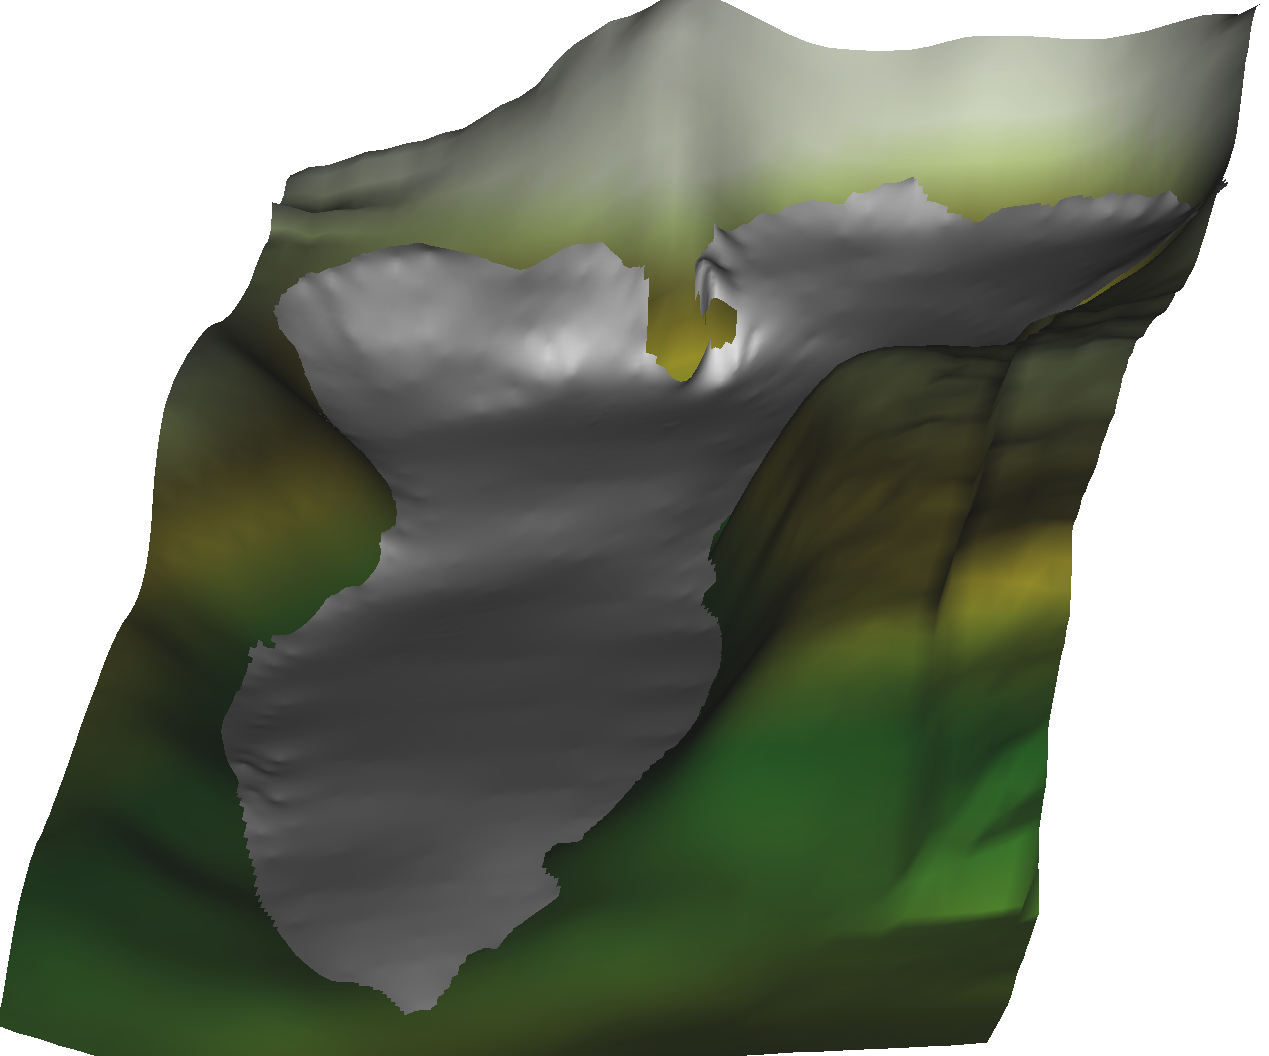
\includegraphics[width=2.75in,keepaspectratio=true]{storglaciaren-dem}
  \caption{Storglaci{\"a}ren, northern Sweden. Left: photo by R. Hock. Right: digital elevation model.}
  \label{fig:storglaciaren}
\end{figure}

To get started run the script \texttt{preprocess.sh} in \texttt{examples/storglaciaren}. It reads the digital elevation model from ASCII files and generates the necessary input files for both the 3-dimensional and the flow-line application. Here we only document the flow-line application.

The mean annual air temperature $T_{\mathrm{MA}}=-6^{\circ}$C at the nearby Tarfala Research Stations serves as the boundary condition for the conservation of energy scheme below the firn line $z_{\textrm{FL}} = 1400$\,m above sea level. Above it, where the ice is temperate, we choose 0$^{\circ}$C. The \texttt{psg_config.cdl} contains parameter choices more suitable for small valley glaciers. Specifically, we increase the limit above which drainge occurs from 1\,\% to 2\,\% liquid water fraction. Furthermore, it sets the till friction angle to 40$^{\circ}$ and the threshold velocity to 10\,m/a.

\texttt{psg_flowline.sh} runs the flow-line application mode. The first two runs smooth the surface and create a more credible enthalpy field. In this example we want to infer the mass balance that has the present day geometry as a steady-state (for now, we ignore the fact that Storglaci{\"a}ren is probably not in a steady-state). As demonstrated in the third run, we can use PISM's mass balance modifier:
\begin{quote}\small
\begin{verbatim}
-surface constant,forcing -force_to_thk psg_flowline_35m_steady.nc -force_to_thk_alpha 0.05
\end{verbatim}
\normalsize\end{quote}
The result of this run is shown in Figure~\ref{fig:storglaciaren-ftt-result}. Without much parameter fine-tuning, simulated surface velocities are reasonably close to observations, c.f. \cite{AschwandenBlatter}.  We also see that a mass balance of about 4 meters per year at the begrschund, almost linearly decreasing to -4.5 meters per year at the tongue, is required to maintain the glaciers geometry. However, observations show that a more realistic present day mass balance decreases lineraly from 2.5 meters per year at the bergschrund to -3 meters per year at the tongue. We now use the surface processes model PSElevation, which is enabled by \texttt{-surface elevation} and allows to define temperature and surface mass balance as a function of surface elevation (see the \emph{PISM's climate forcing components} document for details). The next run uses this present day mass balance which is imposed via 
\begin{quote}\small
\begin{verbatim}
-acab -3,2.5.,1200,1450,1615 -acab_limits -3,0
\end{verbatim}
\normalsize\end{quote} 
For simplicity we assume that the firnline does not change with time. After 25 years the glacier has thinned in the accumulation area but the signal has not yet reached the ablation zone (Figure~\ref{fig:storglaciaren-25a-result}). Plots were produced with the python script \texttt{plot_flowline_results.py}.

\begin{figure}[ht]
  \centering
  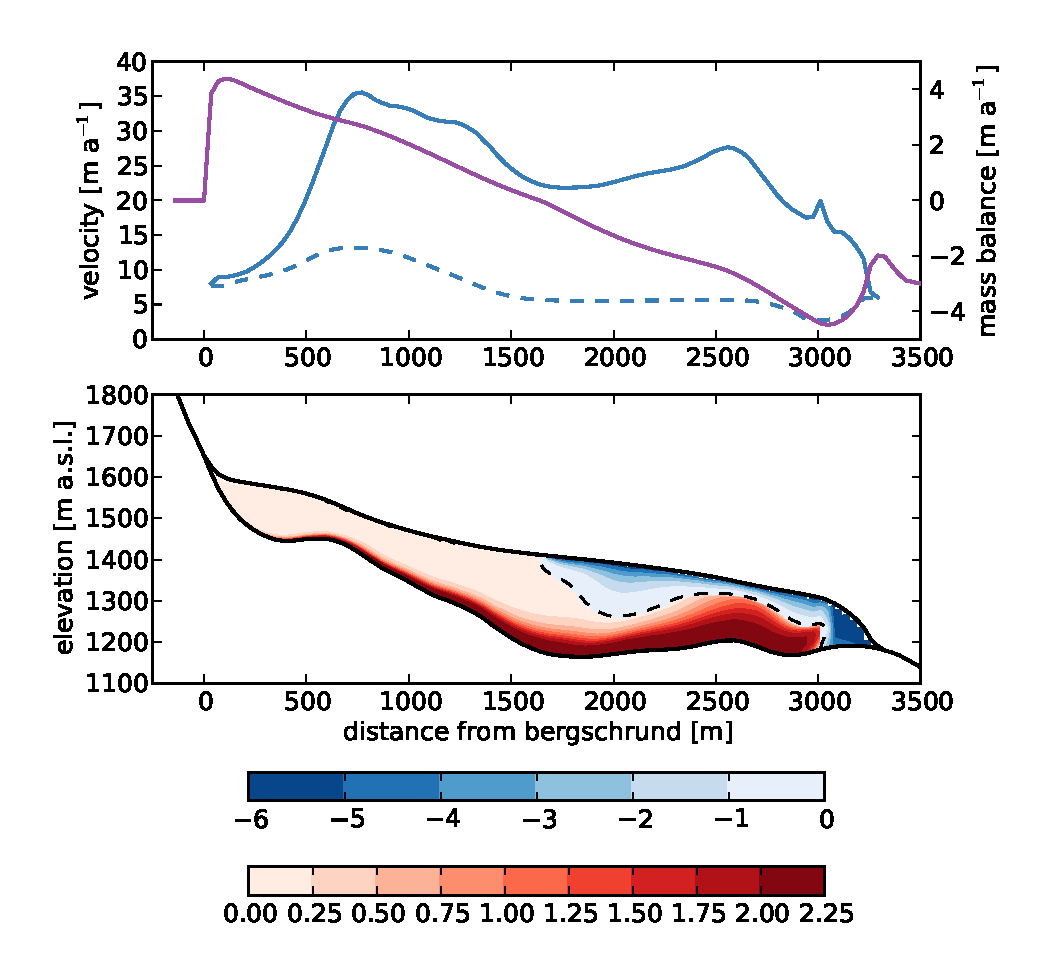
\includegraphics[width=5.in,keepaspectratio=true]{sg-flowline-ftt-result}
  \caption{Storglaci{\"a}ren, northern Sweden.  Modeled present day.  Upper panel: horizontal surface velocity (blue solid), basal sliding velocity (blue dashed), and modified surface mass balance (purple) along flowline in meters per year. Lower panel: thermal structure. Red colors indicate liquid water content, blue colors are temperature in degrees Celsius.}
  \label{fig:storglaciaren-ftt-result}
\end{figure}

\begin{figure}[ht]
  \centering
  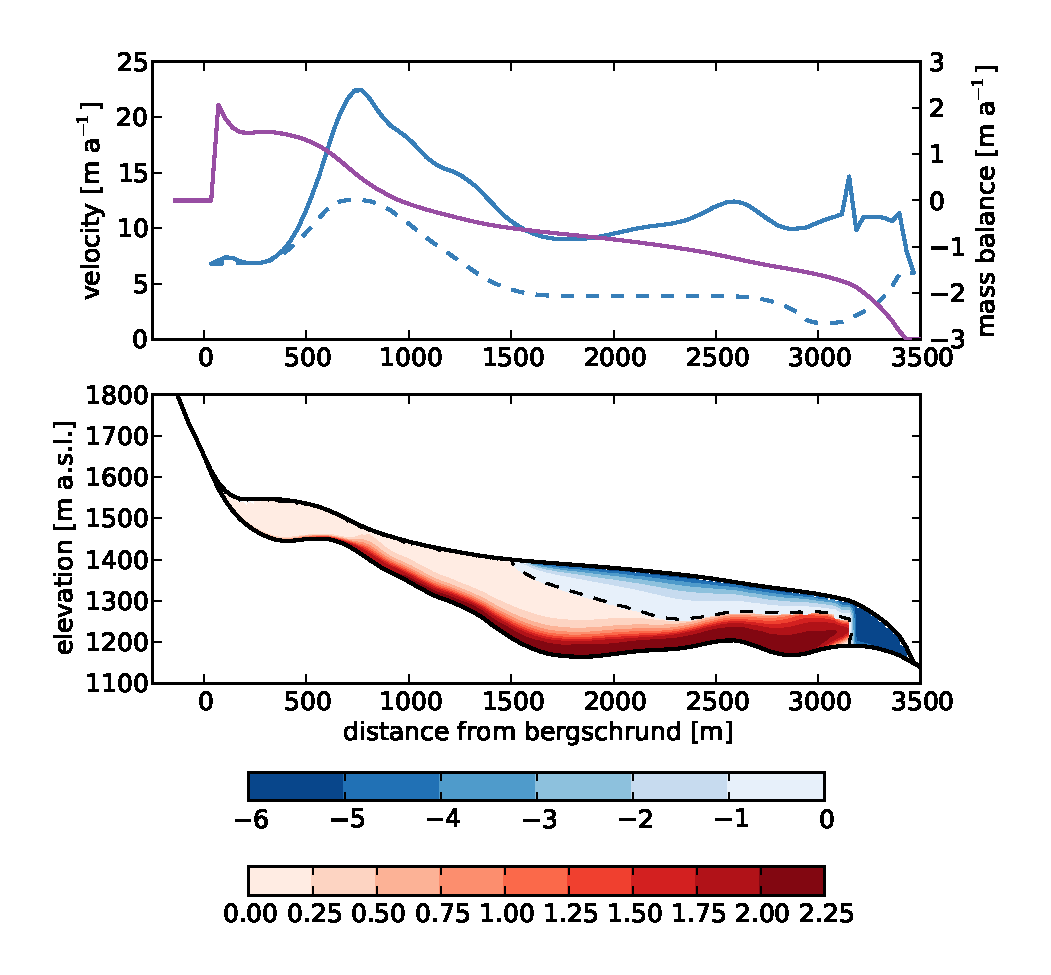
\includegraphics[width=5.in,keepaspectratio=true]{sg-flowline-25a-result}
  \caption{Storglaci{\"a}ren, northern Sweden. 25\,a model run with present-day surface mass balance. Upper panel: horizontal surface velocity (blue solid), basal sliding velocity (blue dashed), and surface mass balance (purple) along flowline in meters per year. Lower panel: thermal structure. Red colors indicate liquid water content, blue colors are temperature in degrees Celsius.}
  \label{fig:storglaciaren-25a-result}
\end{figure}
